% CVPR 2022 Paper Template
% based on the CVPR template provided by Ming-Ming Cheng (https://github.com/MCG-NKU/CVPR_Template)
% modified and extended by Stefan Roth (stefan.roth@NOSPAMtu-darmstadt.de)

\documentclass[10pt,twocolumn,letterpaper]{article}

%%%%%%%%% PAPER TYPE  - PLEASE UPDATE FOR FINAL VERSION
% \usepackage[review]{cvpr}      % To produce the REVIEW version
%\usepackage{cvpr}              % To produce the CAMERA-READY version
\usepackage[pagenumbers]{cvpr} % To force page numbers, e.g. for an arXiv version

% Include other packages here, before hyperref.
\usepackage{graphicx}
\usepackage{amsmath}
\usepackage{amssymb}
\usepackage{booktabs}
\usepackage{float}


% It is strongly recommended to use hyperref, especially for the review version.
% hyperref with option pagebackref eases the reviewers' job.
% Please disable hyperref *only* if you encounter grave issues, e.g. with the
% file validation for the camera-ready version.
%
% If you comment hyperref and then uncomment it, you should delete
% ReviewTempalte.aux before re-running LaTeX.
% (Or just hit 'q' on the first LaTeX run, let it finish, and you
%  should be clear).
\usepackage[pagebackref,breaklinks,colorlinks]{hyperref}


% Support for easy cross-referencing
\usepackage[capitalize]{cleveref}
\crefname{section}{Sec.}{Secs.}
\Crefname{section}{Section}{Sections}
\Crefname{table}{Table}{Tables}
\crefname{table}{Tab.}{Tabs.}


%%%%%%%%% PAPER ID  - PLEASE UPDATE
\def\cvprPaperID{*****} % *** Enter the CVPR Paper ID here
\def\confName{CVPR}
\def\confYear{2022}


\begin{document}

%%%%%%%%% TITLE - PLEASE UPDATE
\title{Detail-Preserving ASCII Art Generation for Images and Videos}

\author{\\
Mateo Estrada\\
University of Texas at Dallas\\
{\tt\small mex210022@utdallas.edu }
% For a paper whose authors are all at the same institution,
% omit the following lines up until the closing ``}''.
% Additional authors and addresses can be added with ``\and'',
% just like the second author.
% To save space, use either the email address or home page, not both
\and
Jacob Jones\\
University  of Texas at Dallas\\
{\tt\small jcj210003@utdallas.edu }
\and
Long Vu\\
University of Texas at Dallas\\
{\tt\small lqv210000@utdallas.edu}
\and
David Wu\\
University of Texas at Dallas\\
{\tt\small dew210000@utdallas.edu}
}
\maketitle

%%%%%%%%% ABSTRACT
\begin{abstract}
   This report is an in-depth discussion and analysis of a video to ASCII conversion algorithm developed as an undergraduate project at the University of Texas at Dallas. ASCII art serves as a unique challenge due to its lack of detail and ties back to early internet forums. It shows that limitation often inspires innovation. Our algorithm features multiple computer vision techniques designed to make the final render as clear and visually pleasing as possible. We will cover such algorithms in the sections of this report, as well as the methods we will use to evaluate the output quality. Our algorithm will be tested on image and video datasets which allow us to collect mathematical evaluation metrics as well as empirical evidence to validate or contradict our claims. The last section of this report will summarize our findings and suggest possible improvements in future attempts.
\end{abstract}

%%%%%%%%% BODY TEXT
\section{Introduction}
\label{sec:intro}





%-------------------------------------------------------------------------


%-------------------------------------------------------------------------
We work on detail-preserving ASCII art because it challenges us to
compress rich visual information into an intentionally constrained
symbolic language without losing the underlying structure or meaning.
ASCII art represents a unique intersection of creativity and
computation, requiring images to be translated into text-based form
while retaining recognizable shapes, edges, and textures. By converting
both images and videos into ASCII, we explore how visual complexity can
be reinterpreted through minimalistic patterns, demonstrating how much
structure can be preserved even when the representational space is
drastically reduced.

The motivation for this project extends beyond novelty. ASCII art serves
as an accessible, low-bandwidth, and platform-agnostic representation,
capable of rendering visual content in environments where traditional
graphics are impractical or impossible. This makes detail-preserving
ASCII generation relevant for embedded systems, terminal-based
interfaces, stylistic rendering, and educational demonstrations of human
perception and compression. More broadly, it exemplifies how innovation
emerges when constraints are embraced and transformed into opportunities
for new forms of expression.

Our technical approach centers on Python as the primary development
environment. We first process images and video frames by segmenting them
into spatial patches and analyzing their local structures. These patches
are then mapped to ASCII characters using multiple conversion strategies
such as luminance-based mapping, edge-aware filtering, and
template-based matching to determine which method best preserves
fine-grained detail. To further enhance structural consistency,
especially in video, we incorporate techniques such as edge
enhancement, temporal smoothing, and noise reduction to mitigate
flickering and instability across frames.

After the conversion stage, all generated ASCII outputs are evaluated
using a quantitative pipeline designed to measure structural fidelity.
The evaluation employs three metrics: Structural Similarity Index
(SSIM), Edge Preservation Ratio (EPR), and Detail Retention Index (DRI).
While SSIM is widely used in image quality assessment, it tends to yield
low values for ASCII outputs due to the inherent change in
representation from pixels to characters. For this reason, our primary
focus is on EPR and DRI, which more accurately capture how well edges
and local details are preserved in a text-based representation. Higher
scores in these metrics indicate that the ASCII output more closely
reflects the structural content of the source image.

Overall, this project aims not only to generate visually coherent ASCII
art but also to systematically study the performance characteristics and
trade-offs of different conversion techniques. By combining
perceptually informed processing, quantitative evaluation, and temporal
stability mechanisms for video, we seek to establish a robust framework
for detail-preserving ASCII art generation that is both creative and
computationally meaningful.

%------------------------------------------------------------------------
\section{Related Work}
ASCII art generation has a long history, originating from early
luminance-based approaches in which pixel intensities were mapped
directly to characters of corresponding brightness
\cite{aalib1997}. These classical methods, popularized in text-rendering
libraries such as AALib, rely on perceptual brightness ordering to
approximate tone but often fail to preserve edges, high-frequency
textures, and spatial structure.

To overcome the limitations of pure luminance mapping, template-based
methods were introduced. These techniques compare local image patches
against pre-rendered ASCII glyph templates using similarity metrics such
as the Sum of Absolute Differences (SAD). Work by Haines
\cite{haines2007ascii} and others demonstrated that template-based
matching provides stronger spatial coherence and captures structural
patterns more effectively than luminance-only methods. However, these
approaches can be sensitive to noise and patch misalignment, often
ignoring the spatial context between neighboring patches. Our method
extends this line of research by incorporating centroid alignment to
achieve more robust patch-to-template comparisons.

Beyond ASCII-specific studies, research in non-photorealistic rendering
(NPR) and image stylization has contributed important insights relevant
to detail preservation. Edge-aware filtering methods, including
bilateral filtering \cite{tomasi1998bilateral} and Difference-of-Gaussians
(DoG) edge enhancement \cite{winnemoller2006realtime}, have been widely
used in sketch rendering, cartoon stylization, and structural
abstraction tasks. These techniques emphasize edge continuity and fine
texture extraction prior to stylization—concepts that directly inform
our preprocessing strategies for ASCII conversion.

In the video domain, maintaining temporal consistency has been an active
area of research. Frame-by-frame stylization methods often suffer from
flickering caused by unstable mappings across consecutive frames.
Ruder et al.\ \cite{ruder2016artistic} addressed this issue in neural
video stylization through optical-flow-guided temporal smoothing,
establishing principles that generalize beyond neural methods. Although
prior ASCII research rarely focuses on video, these works motivate our
temporal smoothing strategy aimed at reducing patch ``bucket switching''
and stabilizing ASCII representation over time.

Overall, while luminance-based mapping and template matching provide
strong foundational approaches for static ASCII generation, relatively
few studies focus on quantitative evaluation or extend these methods to
video. Our work bridges this gap by integrating edge-aware preprocessing,
an improved template comparison pipeline, temporal smoothing techniques,
and a quantitative evaluation framework tailored specifically for
detail-preserving ASCII art generation.


\section{Method}
This project falls into the research-oriented category as
we are developing novel algorithmic approaches to ASCII
art generation with specific focus on detail preservation and
extending these techniques to video processing

\subsection{Template Matching}
During our trials, we will attempt 3 primary techniques for converting image patches into ascii characters. The first of which is called ‘Template Matching’. The idea is that we will pre-render a set of all ascii characters in the same size as our chosen patch size. We will then compare each patch of the input frame to each ascii character template using the Sum of Absolute Differences (SAD) formula. 

\begin{figure}[htbp]
\centering
\[
\sum_{i}\sum_{j} |P[i, j] - T[i, j]|
\]
\caption{SAD Formula. P is the image patch and T is the ASCII template image.}
\label{fig:smoothing}
\end{figure}

Whichever template is closest to the patch will be drawn in the output frame. We can think of this as the ‘naive’ approach, because it assumes that image patches will translate well to a single ascii character. However, there is one obvious issue with this strategy. See figure 1. 

\begin{figure}[H]
\centerline{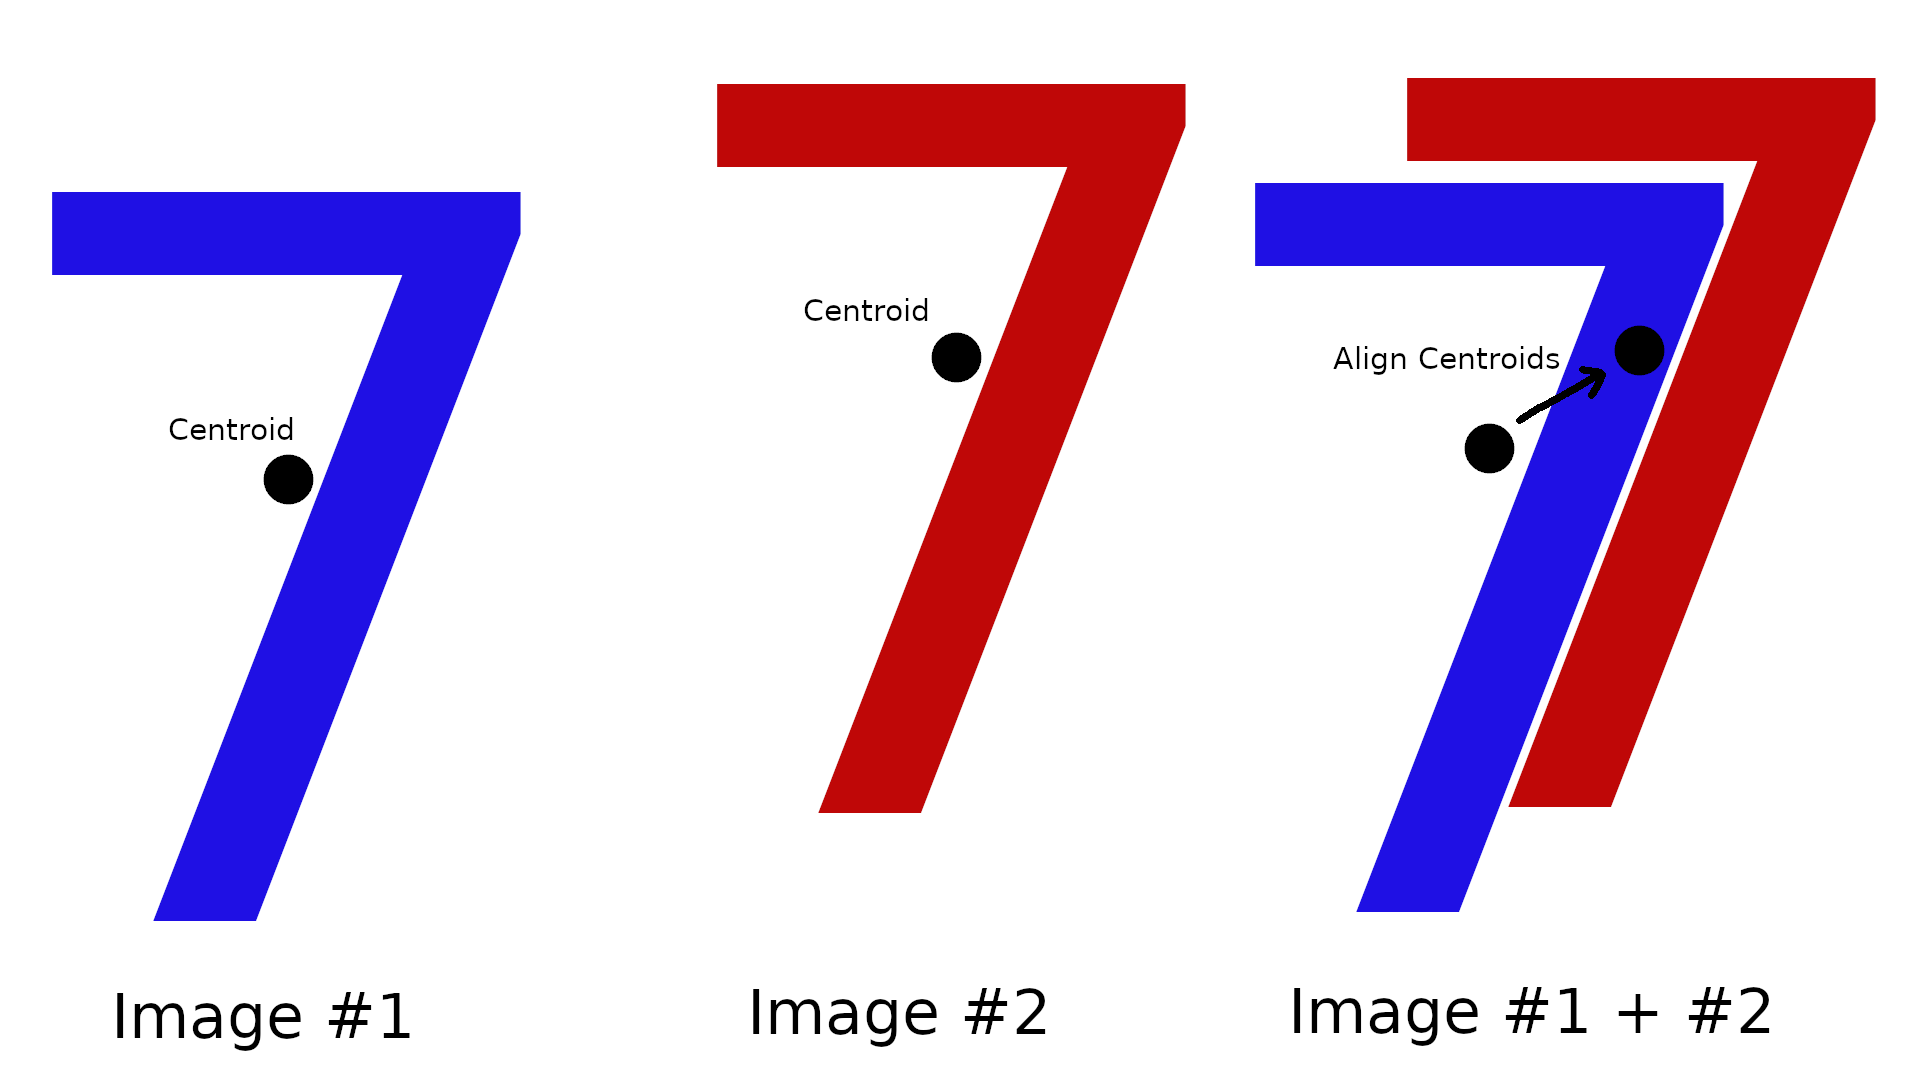
\includegraphics[width=\linewidth]{centroids.png}}
\caption{Training performance graphs: Score over time, Loss, and Average Q-Value.}
\label{fig:graphs}
\end{figure}

In the figure, we can see that image 1 has no overlap with image 2, yet there actual structure is identical. Using SAD would find that these images are a terrible match for each other, but if we replaced image 1 with image 2, it would probably be indistinguishable at a small scale. To solve this issue, we will compute the ‘centroid’ of each template and each patch before comparison. The centroid can be though of as the image's center of mass. It is the average of each pixel in the patch weighted by the intensity of the pixel. Before using SAD, we will shift the patch so its centroid aligns with the template’s centroid. This should allow for a more structural comparison rather than a truly naive comparison.

\subsection{Edge Detection}
empty

\subsubsection{Sobel Filter}
\subsubsection{Difference of Gaussians}
\subsubsection{Edge Consensus}
\subsubsection{Luminance Character Mapping}

\subsection{Temporal Smoothing}
With both luminance matching, template matching, and edge detection, we are essentially taking a patch with many possible values and placing them in a much more restrictive domain. For example, there are only 10 possible characters for 256 luminance values. A suitable term for this process is ‘bucketing’, as we are basically taking each patch and placing it in a bucket that it fits best in. Naturally, if one patch happens to sit on the edge of 2 or more buckets, it could potentially switch between them frequently across multiple frames. This causes a flickering affect which in extreme cases can be highly uncomfortable to look at. We will attempt to reduce this strain by employing a couple different techniques. The first is temporal smoothing. Before running the other ASCII conversion algorithms, we will pre-process the video by taking a weighted sum of each frame and the frame before it\cite{efendi2024}.

\begin{figure}[H]
\centering
\[
S_t = \alpha F_t + (1 - \alpha) S_{t-1}
\]
\caption{Recursive Temporal Smoothing Formula}
\label{fig:smoothing}
\end{figure}

This may introduce ghosting depending on how heavily the previous frame is weighted, but we believe that a small amount of ghosting will not be noticable once converted to ASCII. Another small pre-processing task we will employ is bilateral filtering. Our hypothesis is that a small amount of noise in the input frames will become amplified when converted to ASCII characters. By eliminating noise before conversion, we aim to avoid giving the final video a more cohesive look. We will also make sure to only apply denoising after edge detection as we want to recreate as much edge structure as we can.

\subsection{Evaluation}
empty

\subsubsection{Edge Preservation Ratio}
empty

\subsubsection{Detail Retention Index}
empty

\subsubsection{Temporal Consistency}
empty

\subsubsection{Structural Similarity Index}
empty

\section{Experiments}
\subsection{Data}
Our evaluation will utilize multiple datasets to compre-
hensively assess performance:
\subsubsection{Image Datasets:}
DIV2K High-Resolution Dataset [1]: Contains diverse
high-quality images for testing detail preservation capabili-
ties.
The Unsplash Dataset Lite [3]: Contains various images
sourced from a high amount of contexts and sources to test
various contexts.
\subsubsection{Video Datasets:}
DAVIS Video Segmentation Dataset [2]: Provides anno-
tated video sequences for testing temporal consistency
Real-time Camera Stream: Live webcam input for test-
ing real-time processing capabilities

\subsection{Results}
In our evaluation, we compared luminance-based matching with template matching to determine which method more effectively preserves the edges and perceptual detail in ASCII art generation. The results clearly show that template matching outperforms luminance matching in terms of our evaluation metrics. Template matching achieves this by directly comparing local image patches with character templates, enabling it to capture fine-grained textures, edges, and structural patterns more accurately. In contrast, luminance matching relies solely on brightness values, which fails to account for subtle variations in local texture and often produces characters that do not reflect the underlying image’s spatial details.

\begin{figure}[H]
\centerline{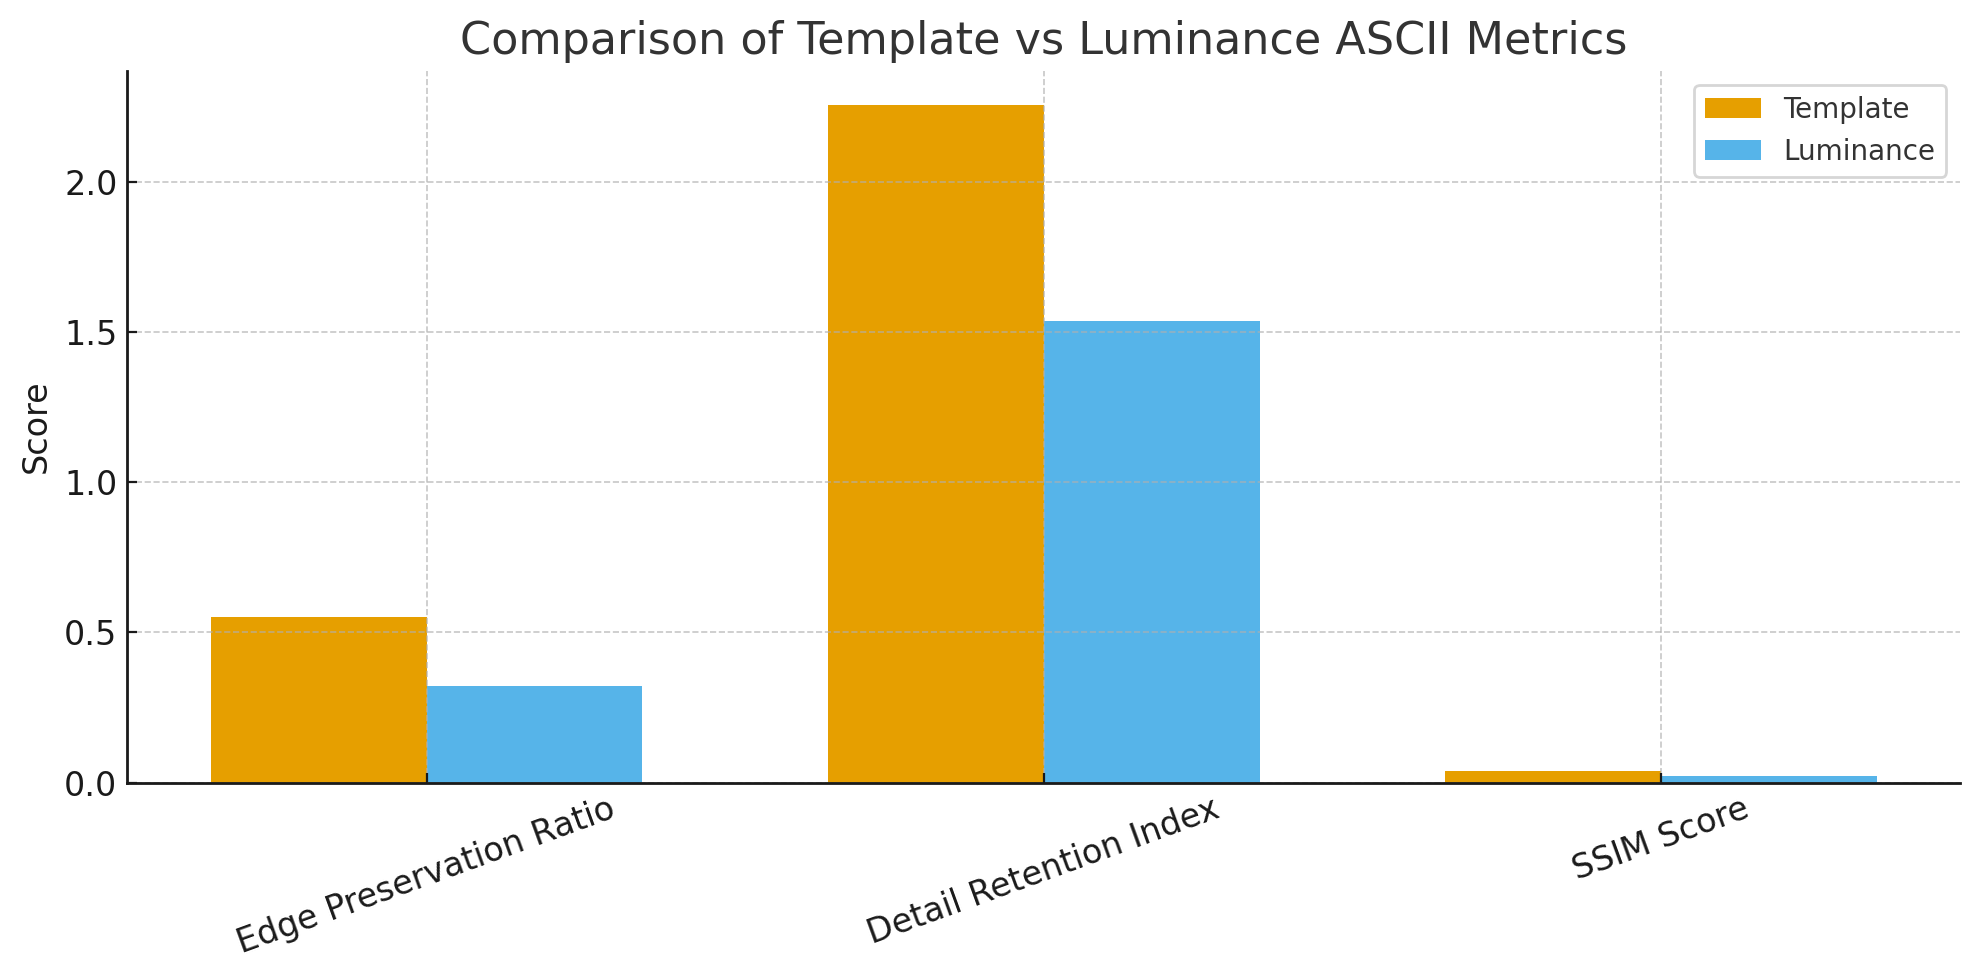
\includegraphics[width=\linewidth]{ChartComp.png}}
\caption{Performance comparison between template mode and luminance mode}
\label{fig:graphs}
\end{figure}

However, this highlights an important insight into what makes ASCII art high quality. Even though template matching scored higher using our metrics, we have found luminance based matching to be the visually superior technique. Template matching compares image patches directly, but it does not take into account average brightness. This leads to most of the image being mapped to bright characters such as the ampersand symbol. This makes the image appear overly bright. When converting images to true ASCII art, you are basically converting to black and white. This means that the wide range of pixel intensities that is normally used to distinguish between objects in an image is completely lost. Luminance based matching attempts to restore this information by leveraging the perceived brightness of a small patch. The bottom line is that tone continuity is more important visually than structure at the pixel level.

\subsubsection{Temporal Consistency}
In this section we’ll show how the techniques discussed in the temporal smoothing section actually improve our conversion algorithm. Using empirical evidence, a reduction in flickering is clear, which heavily contributes to the comfort of the experience. Using our evaluation metrics, we can see that temporal smoothing provides a mathematical improvement to temporal consistency without significantly reducing visual structure.

\begin{table}[H]
\centering
\begin{tabular}{l|cccc}
      &  None & Smoothing  & Denoising & Both \\ \hline
EPR & 0.4402     & 0.4350    & 0.4397  & 0.4334   \\
DRI & 2.0736     & 2.1859     & 2.0612  & 2.1636   \\
TC & 0.5884     & 0.7120     & 0.5903 & 0.7140    \\
SSIM & 0.0172 & 0.0167 & 0.0169 & 0.0164 	\\
\end{tabular}
\caption{Table comparing the effect of temporal smoothing and denoising}
\label{tab:dualheaders}
\end{table}

The numbers show that temporal smoothing has a significant improvement in temporal consistency while keeping other metrics relatively untouched. For reference, the temporal consisteny score of the original video was 0.7841, meaning that temporal smoothing is a highly effective technique. On the other hand, we can see that enabling bi-lateral filtering has only a small improvement in temporal consistency. This is somewhat to be expected. The aim of employing a deniosing algorithm to smooth out flat areas of the image which may appear more scrambled without it. This result can be observed in the slight degredation of the other evaluation metrics, although its effect is likely not significant enough to be noticable in practice.

\subsection{Performance}


\section{Conclusion}
In this project, we explored detail-preserving ASCII art generation for both images and videos, focusing on building a pipeline that balances creativity, computational efficiency, and visual fidelity. Through experiments involving template-based matching, edge-aware filtering, and temporal consistency mechanisms for video, we showed that ASCII art can retain significantly more structure than traditional naïve methods suggest. Our evaluation metrics—particularly the Edge Preservation Ratio (EPR) and Detail Retention Index (DRI)—offered clear quantitative insight into how closely the ASCII results match the original visual content.

A key takeaway from our study is the comparison between template matching and luminance mapping. Although template matching scored higher given our current metrics, luminance mapping had a clear visual appeal that template matching lacked. Luminance mapping preserves a particular quality that template matching and our evaluation metrics failed to consider. The tone continuity of an image is a significant factor in what allows us to perceive form, depth, and contrast, which are essential qualities when you lack the information of color or gray scale images.

Future conversion algorithms using template matching would likely benefit from a pre-processing step to convert input frames to black and white while preserving as much form as possible. Our results also highlight that pure accuracy is not necessarily the only thing that matters. When you are limited in how much detail you can convey, it is important to prioritize the most relevant parts of the image. Therefore, a conversion algorithm might benefit from semantic improvements, such as depth masking to make foreground objects stand out. Object detection could also help the algorithm prioritize giving edge structure to areas of the frame that people already separate subconsciously. A new evaluation metric that measures tone continuity would also go a long way in being able to accurately measure ASCII art quality without empirical evidence.

Overall, our findings show that detail-preserving ASCII generation is both achievable and scalable when grounded in robust strategies and supplemented by modern computer vision techniques. This work not only presents a stronger framework for ASCII art generation but also highlights opportunities for future improvements, including adaptive template libraries, learning-based refinement models, and real-time GPU-accelerated processing. Even within the constraints of text-based representation, our results demonstrate that visually coherent and meaningful depictions can be produced through carefully designed algorithmic pipelines.





%%%%%%%%% REFERENCES
{\small
\bibliographystyle{ieee_fullname}
\bibliography{egbib}
}

\end{document}
